% !TEX TS-program = XeLaTeX
% !TEX encoding = UTF-8 Unicode

\chapter{系统实现}
\label{系统实现}
\defaultfont

\section{系统环境}

\subsection{硬件环境}

\begin{enumerate}
  \item CPU:Intel (R) Core (TM) i7-7700HQ CPU @ 2.80GHz   2.80 GHz
  \item 内存:16.0 GB
  \item 硬盘容量:500GB
\end{enumerate}

\subsection{软件环境}

\begin{enumerate}
  \item 操作系统:Windows 10 家庭中文版(20H2)作为编辑环境+ WSL2(Ubuntu 20.04)作为开发环境
  \item 数据库:mysql Ver 8.0.23-0ubuntu0.20.04.1 for Linux on x86\_64 (Ubuntu)
  \item 客户端:主流浏览器
\end{enumerate}

\section{持久化}
\subsection{Spring Date 和 JPA Hibernate}

\begin{enumerate}
  \item 使用“逻辑模型工具”(例如Navicat Data Module 3)建立模型。
  \item 将模型同步至数据库
  \item 使用IDEA持久化工具生成实体类
  \item 根据逻辑模型为实体类添加注解(实现级联关系)
\end{enumerate}

关键问题如下:

\begin{enumerate}
  \item 多对一,一对多关系实现
        \begin{enumerate}
          \item 方法一:单向 @OneToMany 绑定
          \item 方法二:带有 @JoinColumn 的单向 @OneToMany 绑定
          \item 方法三:双向 @OneToMany , @ManyToOne绑定
          \item 方法四:不带有 ManyToOne 的双向绑定
        \end{enumerate}
        本系统采用第三种方式:在一方类中的多方list加上@OneToMany注解,在多方类中的一方加上@ManyToOne注解。
  \item   级联更新
        \begin{itemize}
          \item 在“一方”(A)中  @OneToMany(cascade = CascadeType.ALL)
          \item “深拷贝”A中的  BCopy = List<B>
          \item 清空A中的  List<B>
          \item  BRepository.deleteAll(BCopy)
          \item  ARepository.save(A)
        \end{itemize}
  \item   级联查询
        \begin{itemize}
          \item Dao层:继承JpaSpecificationExecutor,以及JpaSpecificationExecutor(配合Specification实现复杂查询)实现ARepository。
          \item Service层使用:需要将一个Specification传入aRepository.findAll方法中并实现Specification中的toPredicate方法用于生成查询语句中的where字段,即判断逻辑。
                涉及的重要的类:
                \begin{itemize}
                  \item  javax.persistence.criteria.Path :通过实体类属性名获取字段值
                  \item  javax.persistence.criteria.Join :通过实体类属性名级联
                  \item  javax.persistence.criteria.CriteriaBuilder :拼接生成过滤
                \end{itemize}
        \end{itemize}
\end{enumerate}

% \noindent 关键问题如下:

% \noindent 1.  多对一,一对多关系实现

% \begin{itemize}
%   \item 方法一:单向 @OneToMany 绑定
%   \item 方法二:带有 @JoinColumn 的单向 @OneToMany 绑定
%   \item 方法三:双向 @OneToMany , @ManyToOne绑定
%   \item 方法四:不带有 ManyToOne 的双向绑定
% \end{itemize}

% 本系统采用第三种方式:在一方类中的多方list加上@OneToMany注解,在多方类中的一方加上@ManyToOne注解。

% \noindent 2.  级联更新

% \begin{itemize}
%   \item 在“一方”(A)中  @OneToMany(cascade = CascadeType.ALL)
%   \item “深拷贝”A中的  BCopy = List<B>
%   \item 清空A中的  List<B>
%   \item  BRepository.deleteAll(BCopy)
%   \item  ARepository.save(A)
% \end{itemize}

% \noindent 3.  级联查询

% \begin{itemize}
%   \item Dao层:继承JpaSpecificationExecutor,以及JpaSpecificationExecutor(配合Specification实现复杂查询)实现ARepository。
%   \item Service层使用:需要将一个Specification传入aRepository.findAll方法中并实现Specification中的toPredicate方法用于生成查询语句中的where字段,即判断逻辑。
%         涉及的重要的类:
%         \begin{itemize}
%           \item  javax.persistence.criteria.Path :通过实体类属性名获取字段值
%           \item  javax.persistence.criteria.Join :通过实体类属性名级联
%           \item  javax.persistence.criteria.CriteriaBuilder :拼接生成过滤
%         \end{itemize}
% \end{itemize}

\section{统一返回对象}

使用统一的返回格式不仅可以让接口更漂亮,也可以让前端更方便地处理数据。

\subsection{实现方式}

\noindent 1. 理论前提

为了实现自动格式化,需要一个重要的接口: org.springframework.web.servlet.mvc.meth od.annotationMappingJackson2HttpMessageConverter,该接口允许在执行@ResponseBody或ResponseEntity控制器方法后,但在使用HttpMessageConverter编写响应体之前定制响应。 这正是需要处理返回对象的时机。
具体的实现可以直接注册到RequestMappingHandlerAdapter和ExceptionHandlerExceptionResolver,或者更有可能使用@ControllerAdvice注释,在这种情况下,它们将被两者自动检测到。本系统的实现选择第二种方式:使用@ControllerAdvice注解。

@ControllerAdvice是Spring提供的AOP特性之一,和普通情况下AOP不同在于@ControllerAdvice是由Sping MVC框架织入并提供Web特性。

AOP(面向切面编程)可以使我们在一个地方定义通用功能,但是可以通过声明的方式定义这个功能要以何种方式在何处应用,而无需修改受影响的类\cite{.SpringInAction}。AOP涉及六个概念:
\begin{enumerate}
  \item 通知(Advice):即切面的工作,定义了切面的“什么”和“何时”。
  \item 连接点(Join point):应用程序中可以插入切面的一个个时机。
  \item 切点(Pointcut):定义了切面在“何处”工作,匹配advice要织入的连接点。
  \item 切面(Aspect):为通知和切点的结合。
  \item 引入(Introduction):向现有的类添加新方法或属性。
  \item 织入(Weaving):切面应用到目标对象同时生成代理对象。
\end{enumerate}

\noindent 2. 具体实现

实现ResponseBodyAdvice接口,重写beforeBodyAdvice方法,在该方法中处理封装逻辑。再添加@RestCont rollerAdvice注解(org.springframework.web.bind.annotation.RestCont rollerAdvice,
这是一个方便的注释,它本身由@ControllerAdvice和@ResponseBody注释组成。携带该注释的类型被视为controller advice,其中@ExceptionHandler方法默认使用@ResponseBody语义)。

\subsection{重要问题}

\noindent 1. 问题分析

需要注意的一点是,如果返回对象为String类型时会出现错误:java.lang.ClassCastException :  your response class can not cast to java.lang.String

该问题出现的原因是String类型在ResponseAdvice.beforeBodyWrite()方法中已经被处理为UnifiedResponsor对象,当控制器请求方法的返回类型是String时,用于转换返回值的HttpMessageConverter实例是StringHttpMessageConverter。

\noindent 2. 解决方式

解决方式如图\ref{WebMvcConfigurer}所示:告诉spring框架,不要使用StringHttpMessageConverter来处理控制器方法中的String返回类型,需要在StringHttpMessageConverter前面添加一个MappingJackson2HttpMessageConverter,即代码的第16行。

在运行到15行时(即解决问题之前的情况),处理控制器方法的返回值时使用的转换器序列如图\ref{MessageConverter-list}所示,第二个即为StringHttpMessageConverter。

在写入和刷新响应之前,应该计算ContentLength(当添加http头时)。StringHttpMessageConverter.getContentLength的实现需要传入两个参数,第二参数可选,第一参数为String类型,之后需要调用该参数的getBytes(...).length; 函数的第一个参数为 String 类型,但是返回值已经在ResponseAdvice.beforeBodyWrite()方法中已经被处理为UnifiedResponsor对象,造成参数类型不匹配,抛出ClassCastException。

\begin{figure}[htbp]
  \centering
  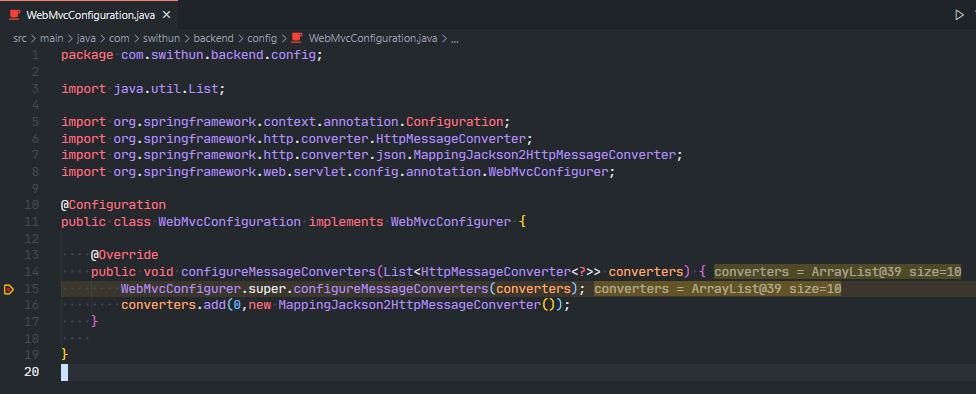
\includegraphics[scale = 0.6]{out/figure/统一返回对象/WebMvcConfiguration-MessageConverter-Code.png}
  \caption{\song\wuhao WebMvcConfigurer}
  \label{WebMvcConfigurer}
\end{figure}

\begin{figure}[htbp]
  \centering
  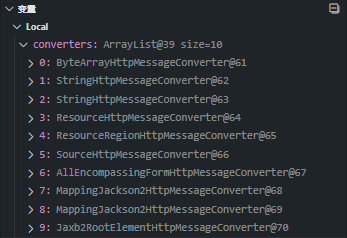
\includegraphics[scale = 0.8]{out/figure/统一返回对象/WebMvcConfiguration-MessageConverter-debug.png}
  \caption{\song\wuhao MessageConverter序列}
  \label{MessageConverter-list}
\end{figure}

之后运行到16行,添加MappingJackson2HttpMessageConverter,添加后如图\ref{MessageConverter-list-after-add}所示,该类继承AbstractJackson2HttpMessageConverter,其中的getContentLength()方法的实现需要哪个传入两个参数,第二个参数可选,第一个参数为Object类型,由于参数不在特定为String类型,所以并不会出现异常。

\begin{figure}[htbp]
  \centering
  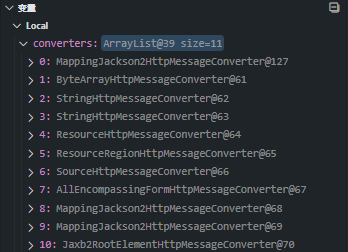
\includegraphics[scale = 0.8]{out/figure/统一返回对象/WebMvcConfiguration-MessageConverter-debug-after-add.png}
  \caption{\song\wuhao 处理后的MessageConverter序列}
  \label{MessageConverter-list-after-add}
\end{figure}


\section{登录与验证授权模块}

\subsection{JWT优势}

随着Web应用规模的逐渐扩大,传统的基于Session和cookie的身份验证技术逐渐显现出它的弊端。
随着服务器的不断增加,由于多个请求可以被分发给不同的服务器,那么此时,服务器该如何确认哪些请求来自同一个用户,对此有两种解决方式
\begin{enumerate}
  \item 多个服务器之间同步用户状态,这样无论用户的请求分发到哪一个服务器,都可以操作用户状态
  \item 判断来自同一个用户的请求,将同一个用户的请求一直分发到同一个服务器
\end{enumerate}
很显然,无论是上述哪种方式,随着用户量的增长开销都会变得很大。
例如第一种方式可以使用会话复制实现,Sesson复制性能也会随着服务器的增加而急剧下降。\cite{.2019h}

JWT(JSON Web Token)的优势在于
\begin{enumerate}
  \item 将用户认证信息保存在客户端,减轻服务器的存储压力。
  \item 提供无状态的身份认证——不需要服务器端多端同步用户状态,利于分布式应用开发。\cite{.2019h}
\end{enumerate}


\subsection{使用JWT与Spring Security 实现验证和授权}

\noindent 关键问题如下:

\noindent 1. 后端配置多用户表使用Spring Security

验证授权涉及到的关键类(图\ref{SpringSecurity}):
\begin{figure}[htbp]
  \centering
  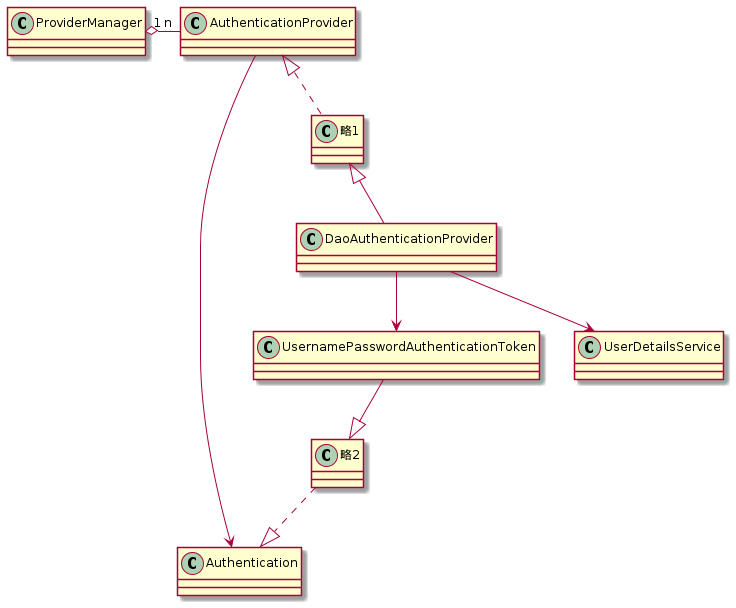
\includegraphics[scale = 0.5]{out/uml/类图/Spring Security/SpringSecurity验证/SpringSecurity验证.png}
  \caption{\song\wuhao Spring Security 验证授权关键类}
  \label{SpringSecurity}
\end{figure}
\begin{enumerate}
  \item  Authentication :用户认证信息。
  \item  UsernamePasswordAuthenticationToken : Authentication 的实现类,用于登录验证,最为常用。
  \item  AuthenticationProvider :认证器,不同的 AuthenticationProvider  处理不同的  Authentication
  \item  DaoAuthenticationProvider : AuthenticationProvider 的实现类,用于处理 UsernamePasswordAuthenticationToken
  \item  ProviderManager :用于管理 AuthenticationProvider
  \item  UserDetailService :为 DaoAuthenticationProvider 提供从数据库查询用户的功能,用于做密码对比。
\end{enumerate}
多用户表配置Spring Security(图\ref{SpringSecurityMultiUser}):
\begin{enumerate}
  \item 为不同用户建立各自的XXXUserDetailService(实现接口UserDetailService),各自的 XXXUserDetailService 从各自的数据库表中查询密码,提供给各自的 XXXDaoAuthenticationProvider 使用。
  \item 为不同用户建立各自的 UsernamePasswordAuthenticationToken
  \item 为不同用户建立各自的 DaoAuthenticationProvider
  \item 进行Security配置:继承WebSecurityConfigurerAdapter并添加注解@Configuration、@EnableWebSecurity和@EnableGlobalMethodSecurity(prePostEnabled = true)

        需要的关键配置:
        \begin{itemize}
          \item 注入 XXXAuthProvider
          \item 向 AuthenticationManager 添加 XXXAuthProvider
          \item 注入 AuthenticationManager
        \end{itemize}
\end{enumerate}
总体流程:
\begin{enumerate}
  \item 前端发起身份验证请求,由于尚未登录,所以前端没有Token信息,因而无法通过Spring Security的验证,这需要在 MySecurityConfig 中配置——放过访问"/authentication"的请求,其他例如注册等不需要验证的 URL 都可以在这里配置,以便进行身份验证和授权。
  \item 请求到达 MyAuthenticationController,此时可以从请求中获取到登录用户身份类型,如果是学生则需要使用 StudentUserDetailService 获取UserDetails,如果是教师则需要使用 TeacherDetailsService 获取UserDetails,同理,如果是管理员则需要使用 AdminDetailsService 获取UserDetials。
  \item 此时进入到 XXXUserDetialsService 中,这里需要重写方法 loadUserByUsername(String username),如果是为学生用户服务的,则需要根据传入的username从学生表中取出用户,如果是为教师服务的,则需要查询教师表并从中找到用户。如果没有找到用户则抛出异常,如果找到了建立 org.springframework.\\security.core.userdetails.User(为UserDetials的实现类)其中包含用户名,用户密码,用户权限和用户身份。
  \item 当获得了 XXXUserDetialsService 返还的 UserDetials,则可以开始进行身份验证。该验证需要 AuthenticationProvider 来完成,因此需要传递需要验证的数据(Authentication)给管理 AuthenticationProvider 的 AuthenticationManager 进行身份验证。由于这里有不同种类的用户且不同种类用户需要查询不同的表,所以需要建立不同 AuthenticationProvider (使用不同的 XXXUserDetialsService(从不同的数据库查询用户))去处理不同的 Authentication,而用来处理用户名用户密码的 AuthenticationProvider 是 DaoAuthenticationProvider,用来处理用户名用户密码的 Authentication 是 UsernamePasswordAuthenticationToken,所以需要为不同用户建立不同的 XXXUsernamePasswordAuthenticationToken 和不同的 XXXAuthProvider。为了绑定 XXXAuthProvider 和 XXXUsernamePasswordAuthenticationToken 则需要重写 XXXAuthProvider 的 supports 方法。
        这个过程中涉及的类比较多且关系比较复杂,可以参考图\ref{SpringSecurityMultiUser}(经过简化,略去了与该流程相关程度不大的类)。
  \item 之后流程又回到了 MyAuthenticationController,此时如果通过了之前的身份验证则可以为用户生成Token了,这里需要使用 JwTokenUtil 生成Token,将 之前获得的 userdetails 传递给 JwTokenUtil,需要注意的是要在 claims 中填入用户角色,这样前端拿到Token之后可以解析出用户角色(这部分信息对应图\ref{jwt}Payload部分)。
  \item 当前端接收到后端的response之后,则可以从返还的Token中获取用户信息存储到localStore。之后的每个请求也都需要在Header中放入Token用于身份验证。
\end{enumerate}
\begin{figure}[htbp]
  \centering
  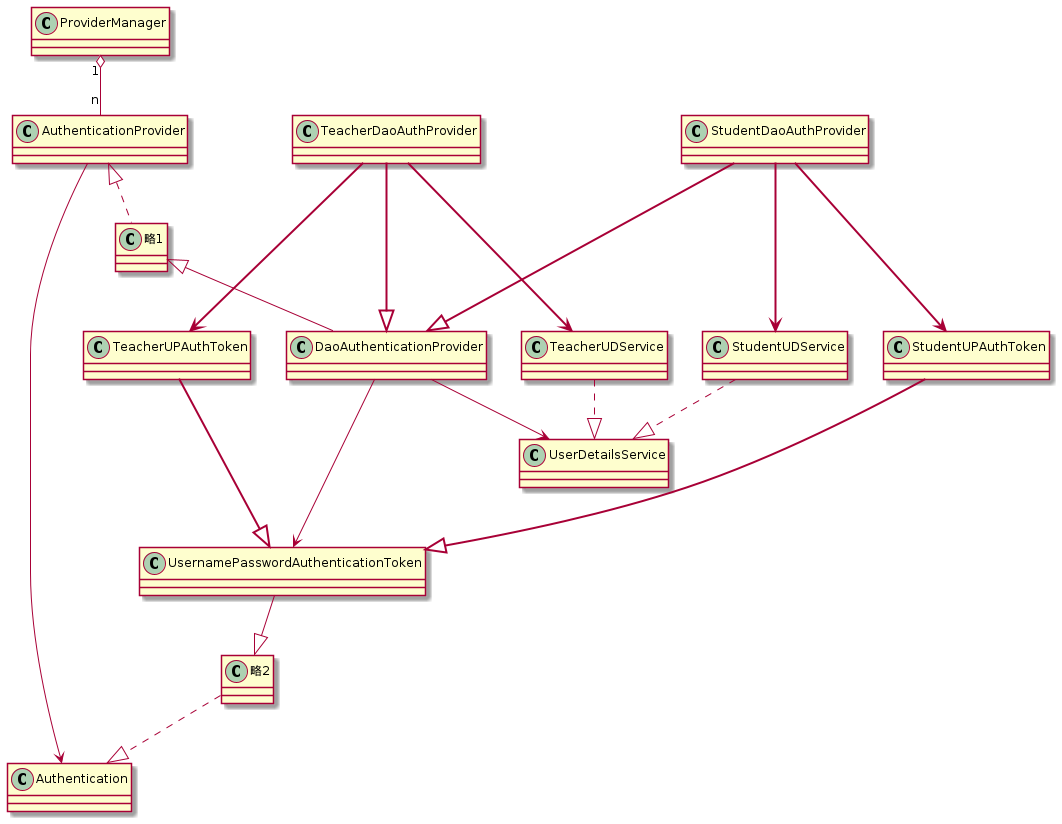
\includegraphics[scale = 0.35]{out/uml/类图/Spring Security/SpringSecurity多用户表验证/SpringSecurity多用户表验证.png}
  \caption{\song\wuhao SpringSecurity多用户表验证}
  \label{SpringSecurityMultiUser}
\end{figure}

\noindent 2. 后端处理CORS跨域问题

CORS(Cross-origin resource sharing)——跨域资源共享,一种可以允许访问其他域名下的受限资源的机制。
目前CORS的现行标准由WHATWG(Web Hypertext Application Technology Working Group)在网络浏览器中实现和测试。\\
CORS-preflight request——预检请求,对于可能会对服务器造成副作用的请求(非简单请求),浏览器会先使用OPTIONS方法发送预检请求
询问服务器是否允许此次跨域请求。\\
简单请求需满足:
\begin{enumerate}
  \item 请求方法:\lstinline[language = xml]| GET、POST、HEAD |
  \item 只使用了如下的安全首部字段,不得人为设置其他首部字段
        \begin{itemize}
          \item Accept
          \item Accept-Language
          \item Content-Language
          \item Content-Type 仅限于text/plain、 multipart/form-data 和 application/x-www-form-urlencoded
          \item HTML头部header field字段仅限于 DPR、Download、Save-Data、Viewport-Width、WIdth
        \end{itemize}
  \item 请求中的任意XMLHttpRequestUpload 对象均没有注册任何事件监听器;XMLHttpRequestUpload 对象可以使用 XMLHttpRequest.upload 属性访问
  \item 请求中没有使用 ReadableStream 对象
\end{enumerate}

总的来说,在CORS问题中涉及两种请求:

\begin{enumerate}
  \item CORS请求:CORS请求是一个包含“Origin”报头的HTTP请求。它不能被可靠地识别为参与了CORS协议,因为所有的方法既不是“ GET ”也不是“ HEAD ”的请求都包含了“ Origin ”头。
  \item CORS preflight请求:也就是所谓的预检请求,是检查CORS协议是否被理解的CORS请求。它使用“ OPTIONS ”作为方法,包括以下 header:
        \begin{enumerate}
          \item  Access-Control-Request-Method :指示将来对同一资源的CORS请求可能使用的方法。
          \item  Access-Control-Request-Headers :指示将来对同一资源的CORS请求可能使用的头。
        \end{enumerate}
\end{enumerate}

OPTIONS方法:用于描述对于目标资源的通信选项。客户端可以放松HTTP OPTIONS 请求来询问 web 服务器支持的 HTTP 方法和其他的选项。如果请求 URL 是一个 ‘*’,那么 HTTP OPTIONS 请求应用于一般的服务器而不是特定的资源。使用HTTP OPTIONS方法的请求应该只检索数据(服务器不能更改其状态)。如果需要更改服务器上的数据,需要使用POST、PUT、PATCH或DELETE方法。

在CORS问题中涉及的响应有两种:\\
第一种对于CORS请求的响应,这种请求可以包含下面的header:
\begin{enumerate}
  \item  Access-Control-Allow-Origin :通过在相应的header中添加被允许的Origin(可以为null也可以为 ‘*’)可以指示哪些响应是否可以被分享。
  \item  Access-Control-Allow-Credentials :指示当请求的凭据模式为"include"时响应是否可以被分享。
  \item  Access-Control-Expose-Headers :通过列出header的名称来指示哪些header可以作为响应的一部分公开。
\end{enumerate}
第二种是对于CORS preflight请求,这种请求可以包含下面的header:
\begin{enumerate}
  \item  Access-Control-Allow-Methods :指示当请求目的为CORS协议时响应的URL支持哪些请求方法。
  \item  Access-Control-Allow-Headers :指示当请求的目的为CORS协议时相应的饿URL支持哪些header。
  \item  Access-Control-Max-Age :表示‘ Access-Control-Allow-Methods ’和  ‘ Access-Control-Allow-Headers ’头提供的信息可以被缓存的秒数(默认为5)。
\end{enumerate}

CORS流程(图\ref{CORS-flow}):

\begin{figure}[htbp]
  \centering
  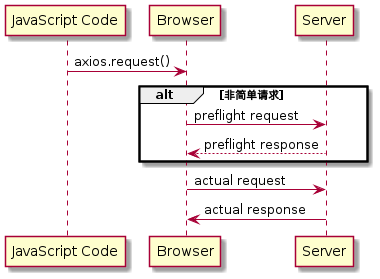
\includegraphics[scale = 0.6]{out/uml/时序图/CORS-flow/CORS-flow.png}
  \caption{\song\wuhao CORS流程}
  \label{CORS-flow}
\end{figure}

Spring Security 配置CORS:

\begin{enumerate}
  \item 打开CORS \begin{lstlisting} [language = Java]
// MySecurityConfig.java
  protected void configure(HttpSecurity httpSecurity) 
                            throws Exception {
    httpSecurity.cors()
              \end{lstlisting}
  \item 配置CORS response:重点的设置有配置允许的请求源(至少需要允许前端服务器的域名前缀);允许的请求方法(类如“GET”,“POST”,“OPTIONS”等);允许的Header(可能涉及的Header都需要配置,至少要允许Access-Control-Allow-Origin)。
\end{enumerate}

\noindent 3. 前端对Token的处理

这里使用Vuex进行管理,为身份验证单独创建一个 auth 模块用于管理身份验证相关的state,action等。
\begin{enumerate}
  \item 在 auth.js 的 state 中: 创建一个 authDate 对象,其中保存用户的Token,refreshToken,tokenExp,userId,userName,userType,以及一个loginStatus。
  \item 在 auth.js 的 getter 中:创建 getLoginStatus() 用于获取用户的登录状态(是否登录),创建 getAuthDate() 用于获取用户的身份信息,创建 isTokenActive() 用于判断 Token 是否过期。
  \item 在 auth.js 的 mutations 中:创建 saveTokenDate() 用于更新 authDate 以及 将 token 保存在浏览器的 localStorage 中。创建 setLoginStatus() 用于更新登录状态。创建 signout() 用于登出 (清除localStorage中的Token,以及将登录状态更改为未登录) 。
  \item 在 auth.js 的 actions 中:创建异步函数 login() 用于登录(使用 axios 发送请求,将 paylaod(username, password, usertype) 放在请求体中发送给后端,使用 mutations 中方法处理返回的结果,成功登录)。
\end{enumerate}

\noindent 4. 前端配置导航守卫

本系统添加全局的前置守卫:使用  router.beforeEach ,该方法接收三个参数,to,from,next(其中第三个参数可选)
\begin{enumerate}
  \item to:想要导航到的规范化格式的目标路由位置。
  \item from:其格式为规范化,表示导航时当前的所在的、正要离开的路由位置。
  \item next:经过判断后应该导航到的路由位置。
\end{enumerate}
配置的导航守卫的大体思路是只要未登录都需要跳转到 login 界面,但是如果访问 login 界面,此时系统尚未登录,然后又会跳转到 login 界面,无限跳转,无法正常工作。所以这里为每个页面的路由设置一个参数 requiredAuth 用于指示该页面是否需要导航守卫。具体设置方法可以选择将 requiredAuth 参数放入路由记录中的路由元信息meta字段中。\\
导航守卫流程:
\begin{enumerate}
  \item 检查 store 中是否保存了 token,如果没有保存则需要从 localStorage 中获取并保存在 store 中。
  \item 调用 auth 模块 中的 isTokenActive getter,从而获知该 Token 是否过期。
  \item 如果 Token 尚未过期并且想要导航到的目标路由需要验证\\meta.requiredAuth === true)则跳转到系统首页,如果并不满足上述条件则需要跳转到 login 页面。
\end{enumerate}

\noindent 5. 为每个请求附带 Token

思路为进行全局配置,在 axios 发送每个请求之前在 Header 中添加 authenticate 字段,其值为登录时从后端获取的 Token。

使用 axios 的 interceptors(拦截器)实现。interceptors 主要可以分成两种:用于处理 request 的 interceptors 和用于处理 response 的 interceptors。由于是需要在发送请求时添加 Header ,所以选择第一种,配置其config(config.headers.common.Authorization = `bearer \${authData.token}`),其中 token 可以从 store 中获取。

这里需要注意的一点是,由于许多请求不是简单请求,会触发上文提到的 CORS 问题,对于 CORS preflight 请求的响应中,系统后端会配置允许 Authorization 字段,但是如果访问其他网站,该字段可能会不被允许,造成访问失败,所以可以在 interceptors 中根据访问的 url 选择是否需要添加 token(其中 url 可以从 config 中获取)。

\section{Jackson序列化时无限递归问题}

当实现级联关系时选择双向绑定会造成 Jackson 序列化时无限递归问题。

例子(省略其他相关性不大的代码):

\begin{lstlisting} [language = Java]
public class A {
  private Integer id;
  private List<B> bs;
}
\end{lstlisting}

\begin{lstlisting} [language = Java]
public class B {
  private Integer id;
  private A a;
}
\end{lstlisting}

对应的数据库表\ref{jackson-A}和\ref{jackson-B}所示。

\begin{table}[htbp]
  \begin{minipage}{0.45\linewidth}
    \centering
    \song\wuhao
    \caption{jackson-A}
    \label{jackson-A}
    \begin{tabular}{l}
      \hline
      A的id \\ \hline
      id    \\ \hline
    \end{tabular}
  \end{minipage}
  \begin{minipage}{0.45\linewidth}
    \centering
    \song\wuhao
    \caption{jackson-B}
    \label{jackson-B}
    \begin{tabular}{ll}
      \hline
      B的id & A的id \\ \hline
      id    & A\_id \\ \hline
    \end{tabular}
  \end{minipage}
\end{table}

关于Jackson需要知道的两个概念:
\begin{enumerate}
  \item 序列化:从实体对象映射为Json对象
  \item 反序列化:从Json对象映射为实体对象
\end{enumerate}

如果现在获取A,序列化A的时候会序列化bs,而bs中的每一个B对象都需要序列化A,此时会造成无限序列化。

三种解决方式:
\begin{enumerate}
  \item 使用 @JsonManagedReference 和 @JsonBackReference\\
        @JsonManagedReference(com.fasterxml.jackson.annotation.JsonManagedReference)\\
        @JsonBackReference(com.fasterxml.jackson.annotation.JsonBackReference)\\
        Managed用于“一方”,即A中的List<B>,Back用于“多方”,即B中的A,表示能从A方找到B,但是无法从B方找到A。
  \item 使用 @JsonIgnore\\
        @JsonIgnore(com.fasterxml.jackson.annotation.JsonIgnore)\\
        第一种方法的问题是,序列化时A会序列化List<B>,B不会序列化A,如果此时想要A不序列化List<B>,B序列化A就无法做到。可以将@JsonIgnore注解加载List<B>上从而实现。
  \item 使用 @JsonProperty(access = ...)\\
        @JsonProperty(com.fasterxml.jackson.annotation.JsonIgnore)\\
        前两种方法在序列化和反序列化时的效果都相同,但是如果此时的需求是前端发过来的json对象映射为B时需要映射a属性,但是发送给前端json对象时不需要映射a属性(防止造成无限递归序列化)时可以设置JsonProperty.access(),序列化对应read,反序列化对应write,共有四种选择:
        \begin{enumerate}[label=\circled{\arabic*}]
          \item AUTO
          \item READ\_ONLY
          \item READ\_WRITE
          \item WRITE\_ONLY
        \end{enumerate}
        选择第四种方式即可实现,即在B类中的A类型对象加上注解 @JsonProperty(access = JsonProperty.Access.WRITE\_ONLY)
\end{enumerate}

\section{文件上传模块}

\noindent 1. 前端配置

前端使用 Element Plus 的上传组件

关键配置参数:
\begin{enumerate}[label=\circled{\arabic*}]
  \item action:上传的地址,即后端定义的接口。
  \item multiple:设置可以多选文件。
  \item on-suscess:文件上传成功时的钩子。
  \item on-preivew:点击文件列表中已上传的文件时的钩子。
  \item on-remove:	文件列表移除文件时的钩子。
  \item auto-upload:是否在选取文件后立即进行上传。
  \item data:附带的数据,这里放入文件名字。
  \item file-list:文件列表数据。
\end{enumerate}

\noindent 2. 后端配置

\begin{enumerate}
  \item Controller:\\
        文件上传函数使用 @PostMapping 注解,接受两个参数,其中 MultipartFile file 用来映射文件,Principal principal 用于从中取得发送请求的用户信息。
  \item Service:
        创建处理函数,共接受两个参数(文件和用户名),当存储文件时共需要四个信息:
        文件名字:从 file 中可以提取出文件名;
        拥有该文件的学生姓名:从 principal 中可以获取;
        文件数据:file.getBytes();
        文件类型:file.getContentType();
        至此,存储一个文件的所有信息已经获得,通过这些信息新建一个文件实体对象,使用文件Repository存储文件。
\end{enumerate}

\section{文件更新模块}

\noindent 1. 前端功能实现:
\begin{enumerate}[label=\circled{\arabic*}]
  \item 文件更新页面 template 部分

        需要一个input,将其 type 设置为 file,由于需要修改样式,要为 input 添加 label,作为文件更新按钮,其中 input 的 id 不能静态绑定,因为在文件更新按钮的外层使用了 v-for 遍历文件,如果所有 id 都是静态绑定的,将造成不论点击那一按钮,更新的都是文件列表的第一个文件,所以这里需要使用动态绑定“:id“方式,由于文件的id都是唯一的,刚好可以与 input 的 id 绑定。
  \item 更新文件函数(前端处理部分):

        创建文件更新函数,要做的是事情有:
        \begin{enumerate}
          \item 获得文件 const file
          \item 新建 Form 表单
          \item 为表单填入文件,文件id,文件名
          \item 新建请求配置,配置 Content-Type 为 multipart/form-data
          \item 调用更新文件函数(传入参数文件和配置)
        \end{enumerate}
  \item 更新文件函数(与后端交互交互部分):

        这部分的异步代码交由Vuex管理,可以在多个模块中重复使用,逻辑为将传入的 form 表单作为请求体,传入的 config 作为请求配置向后端发起请求传送文件。
\end{enumerate}
\noindent 2. 后端功能实现:
\begin{enumerate}
  \item Controller:
        使用 MultipartFile file 映射新上传的文件,使用 Integer id 映射需要被更新的文件的 id,将两个参数传递给Service 处理。
  \item Service:
        首先从数据库取出原文件,更新文件的名称,文件的类型,文件的数据,之后重新保存回数据库。
\end{enumerate}

\section{文件下载模块}

\noindent 1. 前端请求函数:

使用 axios 发送 get 请求,参数为文件id,responseType 为 blob 类型。

这里的重点是改变XMLHttpRequest对象的 responseType属性,将其设置为 “blob”,否则返回的数据会被解析为 Json 对象,无法正确地处理文件,导致文件乱码。

\noindent 2. 后端处理函数:

处理函数接收一个参数即文件id, 这里需要注意两点,

第一点是一定要设置 response 的 Content-Type为“application/pdf”,设置方法为在 @GetMapping注解中 将 produces 参数赋值为“application/pdf”。

第二点是因为本系统配置了统一返回对象,会对返回值在发送前进行封装,这次封装会导致返回的值不再是文件数据本身,所以需要设置不对 byte[] 类型进行重新封装。

\section{文件评论模块}

由于评论模块在学生页面和教师页面都需要使用,所以这里将评论功能抽出为一个组件。评论的结构是树形结构,选择对Element UI中的树形组件进行二次封装为一个组件。

新建一条评论需要四个属性,评论id(回复哪一条评论,如果为空则表示新建一条评论),文件id(表示在哪篇论文下评论),评论人,评论内容。

在data()中建立fileId,commentId对象,和组件进行绑定,这样在选择文件和选择评论时就可以记录这两个属性。评论内容只需要将input和commentData中的comment属性绑定就可以获得。

至于最后一个属性——评论人,在后台Controller接收到请求后利用Principal便可以获得发送请求的用户信息,至此四个属性全部获得便可以存储到数据库。

\section{文件预览模块}

\noindent 1. 前端部分
\begin{enumerate}
  \item 实现PDF预览:编写WebViewer组件,放入一个弹窗,使用文件下载模块的前端请求函数从后台获取文件的blob对象,通过双向绑定的方式将对象传入WebViewer组件实现pdf预览和操作。
  \item 实现点击不同文件按钮弹窗显示不同PDF:由于WebViewer组件每次mount的时候会在同一个element上再新建一个实例,会出现错误,所以选择每次点击按钮时获取不同的PDF blob对象,显示弹窗时重新渲染WebViewer组件。
  \item 实现组件重新渲染:实现组件重新渲染的方式有三种
        \begin{itemize}
          \item 使用 this.\$forceUpdate() (适合vue2)
          \item 使用 v-if (不符合目前逻辑)
          \item 使用 :key (符合逻辑且可实现)
        \end{itemize}
        选择第三种方式,当使用key时,当key发生变化,组件会基于 key 的变化重新排列元素顺序,并且会移除/销毁 key 不存在的元素,即会完整地触发组件的生命周期钩子。
\end{enumerate}
\noindent 2. 后端部分:同文件下载模块后端处理。


\section{统计模块}

统计数据由后台生成,传递给前台使用JavaScript可视化工具——Echarts展示。


\section{本章小结}

本章主要介绍了在系统实现过程中的主要模块的实现,关键问题的解决。其中关键问题的解决对系统的稳定性,可维护性的提升都有很大的帮助。